% ------------------------------------------------------------------
% Fig. 2 -- Search loop.
%
% Same idiom as Fig. 1 (standalone document, grayscale fills, chunky
% grey flow arrows, bold caption set outside the nodes) -- black and
% white throughout, no color, per print-format requirement.
% The iterative part is a compact ring inside a dashed boundary, so the
% return edge spans one row gap instead of sweeping back across the
% whole figure. Wording avoids "surrogate" throughout -- boxes name
% what is being fit ("model") or how a quantity is obtained
% ("predicted" / "simulated") instead.
%
% Compile on its own:  tectonic -X compile figures/fig_search.tex
% ------------------------------------------------------------------
\documentclass[tikz,border=5pt]{standalone}
\usepackage{amsmath,amssymb}
\usetikzlibrary{positioning,arrows.meta,calc,fit,backgrounds}

\begin{document}
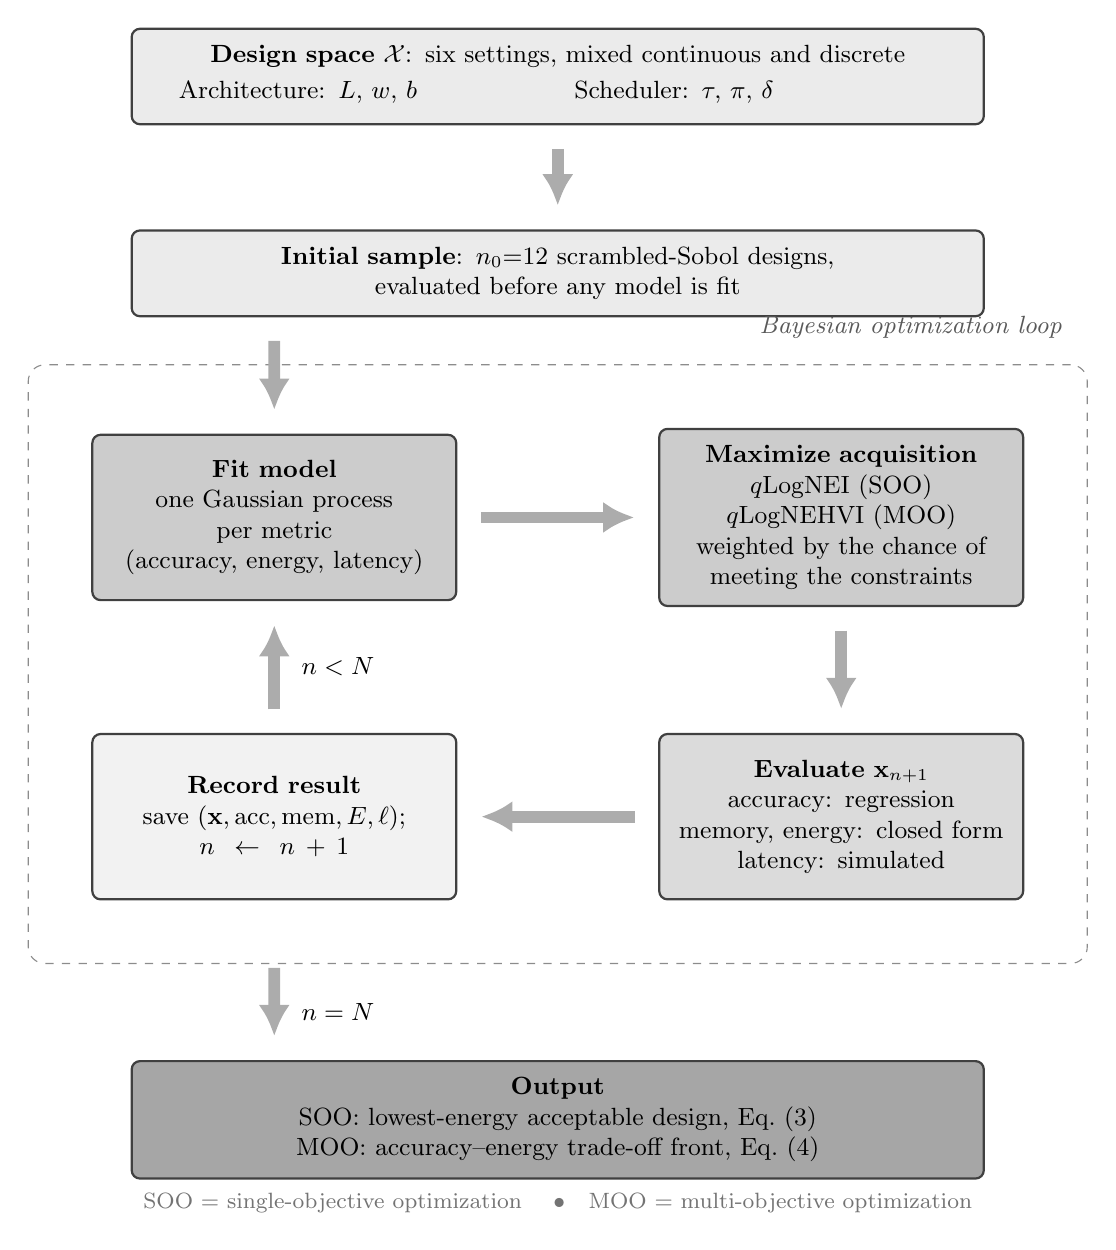
\begin{tikzpicture}[
    thick,
    font=\small,
    blk/.style   = {rounded corners=3pt, draw=black!75, align=center,
                    inner sep=6pt},
    wide/.style  = {blk, text width=104mm},
    loopbox/.style  = {blk, text width=42mm, minimum height=21mm},
    stage/.style = {font=\normalsize\bfseries, text=black!75, align=center},
    lbl/.style   = {font=\small\itshape, text=black!65},
    arrow/.style = {>={LaTeX[width=4mm,length=4mm]}, ->, line width=1ex,
                    gray!65, shorten <=3mm, shorten >=3mm},
    elbl/.style  = {font=\small, text=black, inner sep=2pt},
  ]

% ---------- entry ---------------------------------------------------
\node[wide, fill=black!8] (space) at (0, 6.8)
     {\textbf{Design space} $\mathcal{X}$: six settings, mixed
      continuous and discrete\\[2pt]
      \begin{tabular}{@{}p{46mm}p{46mm}@{}}
      Architecture: $L,\,w,\,b$ & Scheduler: $\tau,\,\pi,\,\delta$
      \end{tabular}};
\node[wide, fill=black!8] (init)  at (0, 4.3)
     {\textbf{Initial sample}: $n_0{=}12$ scrambled-Sobol designs,\\
      evaluated before any model is fit};

% ---------- the loop, as a ring inside a dashed boundary ------------
\node[loopbox, fill=black!20] (gp)  at (-3.6, 1.2)
     {\textbf{Fit model}\\ one Gaussian process\\ per metric\\
      (accuracy, energy, latency)};
\node[loopbox, fill=black!20] (acq) at ( 3.6, 1.2)
     {\textbf{Maximize acquisition}\\ $q$LogNEI (SOO)\\ $q$LogNEHVI (MOO)\\
      weighted by the chance of\\ meeting the constraints};
\node[loopbox, fill=black!14]   (ev)  at ( 3.6,-2.6)
     {\textbf{Evaluate} $\mathbf{x}_{n+1}$\\ accuracy: regression\\
      memory, energy: closed form\\ latency: simulated};
\node[loopbox, fill=black!5]  (upd) at (-3.6,-2.6)
     {\textbf{Record result}\\ save $(\mathbf{x},\mathrm{acc},\mathrm{mem},
      E,\ell)$;\\ $n \leftarrow n+1$};

\begin{scope}[on background layer]
\node[draw=black!45, dashed, rounded corners=6pt,
      fit=(gp)(acq)(ev)(upd), inner sep=8mm] (ring) {};
\end{scope}
\node[lbl] at (ring.north east)
     [anchor=south east, xshift=-2mm, yshift=2mm]
     {Bayesian optimization loop};

% ---------- exit ----------------------------------------------------
\node[wide, fill=black!35] (out) at (0,-6.45)
     {\textbf{Output}\\ SOO: lowest-energy acceptable design, Eq.~(3)\\
      MOO: accuracy--energy trade-off front, Eq.~(4)};

% ---------- the flow ------------------------------------------------
\draw[arrow] (space) -- (init);
\draw[arrow] ([xshift=-3.6cm]init.south) -- (gp.north);

\draw[arrow] (gp)  -- (acq);
\draw[arrow] (acq) -- (ev);
\draw[arrow] (ev)  -- (upd);
\draw[arrow] (upd.north) -- node[elbl, right=2mm] {$n<N$} (gp.south);

\draw[arrow, shorten <=0.5mm] (ring.south -| upd) -- node[elbl, right=2mm] {$n=N$}
             ([xshift=-3.6cm]out.north);

\node[font=\footnotesize, text=black!55] at (0,-7.5)
     {SOO = single-objective optimization \quad$\bullet$\quad
      MOO = multi-objective optimization};

\end{tikzpicture}
\end{document}
